\documentclass{article}
\usepackage{tikz}
\usetikzlibrary{shapes.gates.logic.US}
\usetikzlibrary{circuits.ee.IEC}


\title{Assignment 1 | FPGA Lab}
\author{EE22MTECH02005}
\date{January 2022}

\begin{document}


\maketitle

\section{Question}
Write the Boolean Expression for the result of the logic circuit as shown below:
 
    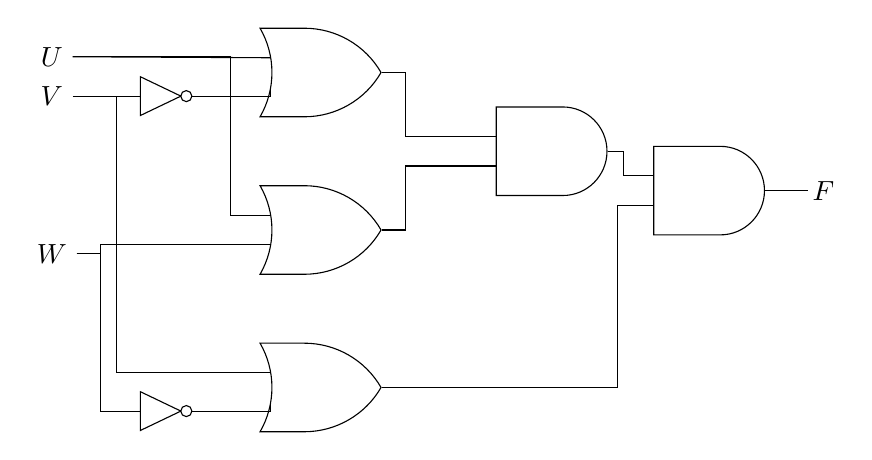
\begin{tikzpicture}[ circuit symbol wires]
    \node (x) at (-1.8,4.7) {$U$};
    \node (y) at (-1.8,2.2) {$W$};
    \node (z) at (-1.8,4.2) {$V$};
    \node[or gate US, minimum size=32pt, draw] at (1.5,0.5) (or1) {};
    \node[or gate US, minimum size=32pt, draw] at (1.5,2.5) (or2) {};
    \node[and gate US, minimum size=32pt, draw] at (4.5,3.5) (And21) {};
    \node[or gate US, minimum size=32pt, draw] at (1.5,4.5) (or3) {};
    \node[and gate US, minimum size=32pt, draw] at (6.5,3) (And22) {};
    \node[not gate US, minimum size=12pt, draw] at (-0.5,0.2) (not1) {};
    \node[not gate US, minimum size=12pt, draw] at (-0.5,4.2) (not2) {};
    \draw (y.east) - ++(right:3mm) |- (not1.input);
    \draw (y.east) - ++(right:3mm) |- (or2.input 2);
    \draw (x.east)-- (or3.input 1);
    \draw (x.east) - ++(right:2cm) |- (or2.input 1);
    \draw (z.east) - ++(right:5.5mm) |- (or1.input 1);
    \draw (z.east) - ++(right:3mm) -- (not2.input);
 
   \draw (not1.output) -| (or1.input 2);
   \draw (not2.output) -| (or3.input 2);
   \draw (or3.output) - ++(right:3mm)|- (And21.input 1);
   \draw (or2.output)- ++(right:3mm) |- (And21.input 2);
   \draw (And21.output)- ++(right:2mm) |- (And22.input 1);
   \draw (or1.output)- ++(right:3cm) |- (And22.input 2);
    \node (z) at ($(And22) + (1.5,0)$) {$F$};
   \draw (7.26,3) -- (7.8,3);
    \end{tikzpicture}

\section{Solution}

F = $(U + \bar{V})$.($U+W$).($V+\bar{W}$)

\end{document}